\chapter{Sources of Learning Data Science}
Data science skills are straightforward to obtain, they need experience and learning. Nowadays there are many online and offline which teaches them in detail. While some prefer online courses such as Coursera or Udacity, some prefer to go to universities for a year or two-year long dedicated courses. Let's look at what are the most popular sources of learning data science among the respondents of the kaggle survey. In this question, one participant could have chosen multiple choices, hence the x-axis represents "percentage" of respondents who selected a particular choice.

\begin{figure}[!htpb]
    \centering
    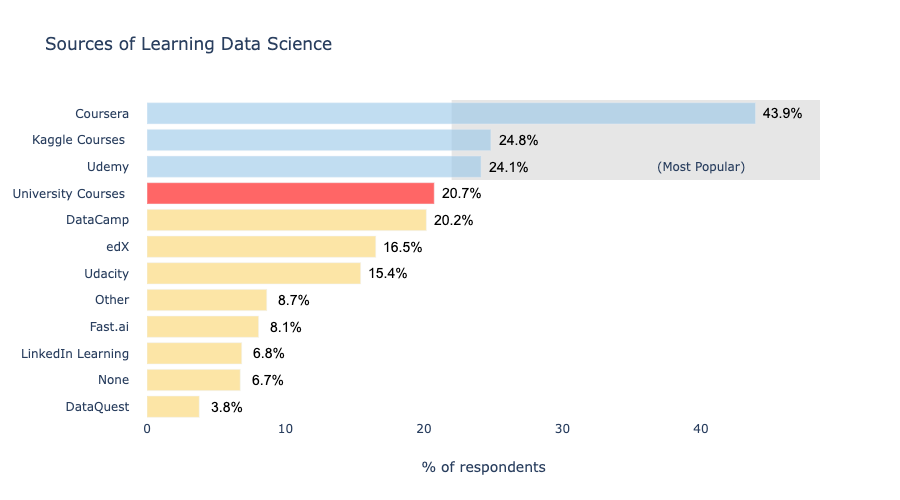
\includegraphics[width=\linewidth]{Figures/Outputs/sources.png}
    \caption[Sources of learning]{Sources of learning.}
    \label{fig:figure-01}
\end{figure}

\subsubsection{Key Findings}
\begin{enumerate}
    \item About 44\% of the respondents selected "Coursera" as the primary source of learning data science. Coursera is the popular online learning platform which provides both free courses and paid specializations.
    \item Coursera and its founder \href{https://en.wikipedia.org/wiki/Andrew_Ng}{Andrew NG} have made very significant contributions to the data science revolution. Back in 2012, Andrew NG released the very popular Machine Learning course which became the first choice for many to learn data science. In 2017, \href{https://www.deeplearning.ai/}{Deeplearning.ai} was launched and it became very popular data science specialization. These courses and many others from well known academic names on the online platform makes Coursera as the primary choice among the data science enthusiasts.
    \item \href{https://www.kaggle.com/learn}{Kaggle Learn} was selected by almost one-fourth of the respondents. Kaggle team launched these courses somewhere around early 2017. They are composed of notebook style materials which not only focusses on teaching the concepts but also the programming part as well.
    \item Then there are other sources such as Udemy, Udacity, edX, fast.ai etc. These platforms als provide online materials and courses to learn data science.
    \item Then there is a group of individuals who prefer to go to a university to pursue higher education degrees. Among the survey participants, about \textbf{one-fifth of the participants} had completed university degrees. Accoding to multiple sources ( \href{https://www.master-and-more.eu/en/7-reasons-why-you-should-choose-a-masters-degree/}{Masters-And-More}, \href{https://www.careeraddict.com/masters-degree-benefits}{CareerAdditct}, \href{https://www.mybaggage.com/blog/why-do-a-masters-degree-the-pros-and-cons/}{MyBaggage} ) different individuals have many different reasons to choose university courses over online courses. The most common are:
    \begin{itemize}
        \item Personal Goal
        \item Better Salary
        \item Gain More Knowledge
        \item Better Job Roles
        \item Career Change
    \end{itemize}
\end{enumerate}

\section{Designing My Survey}
I created my own survey to know the student's choices this question and shared it in several groups associated with National University of Singapore. I managed to get about 120 responses from different people for this survey. Following is the response distribution of the Question.

Link of the Survey: \href{https://docs.google.com/forms/d/19ov_EmBVdwc70tPUoylm8gPNz2bK4j21UAirDcQHB_Q/viewform?edit_requested=true}{Survey} 

Link of the Responses: \href{https://docs.google.com/spreadsheets/d/1OG9IBYNzcb0dlDBI9egI2PynSoH8gpCFv_CrvDVyHPE/edit?usp=sharing}{Responses}

\note {Names are removed to maintain the privacy of the individuals.}

\begin{figure}[!htpb]
    \centering
    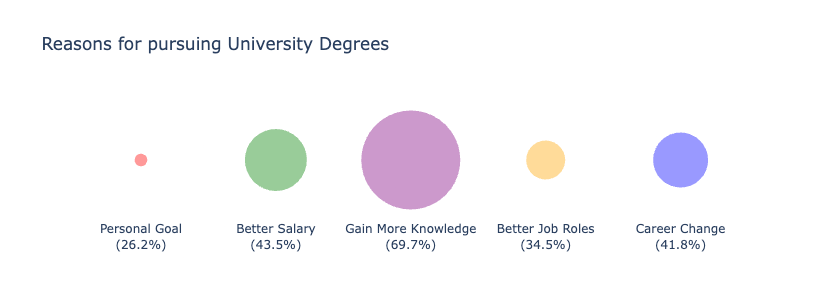
\includegraphics[width=\linewidth]{Figures/Outputs/reasons-for-study.png}
    \caption[Reasons for pursuing university degree]{Reasons for pursuing university degree.}
    \label{fig:figure-02}
\end{figure}

\subsubsection{Key Findings}
\begin{enumerate}
    \item Most of the people decided to pursue higher education degrees to gain more knowledge. This was the primary reason for about 70\% of the individuals who were part of this survey. Every two out of five people decided to pursue university degrees to get better salaries or to change their professions. Only about one-fourth of individuals had their own personal goal to go for a university degree.
    \item If we just look at the number of individuals who selected "gain more knowledge", the same but important question arises again: "Is it worth spending a huge amount of money to gain knowledge that one can get from free sources?" Arent' the free online sources good enough to gain more knowledge. Or, Can't these sources provide enough skills and knowledge to get that better salary, better job roles, or provide a pathway for a career change.
    \item The interesting fact to note that most of the online courses on Coursera, Udemy etc. are also from the same universities or the same professors. Many of them are free as well. So if "gaining more knowledge" is the only goal then it is worth considering these free courses.
\end{enumerate}

\section{The Academic Landscape}
Whatever be the debate but one point is definitely clear, Universities across the globe do benefit a lot from this increased interest in higher education degrees. Many universities have now started specialized masters degree programs in analytics, data science, business analytics etc. The following chart shows some of the popular master's degree programmes from US universities along with their tuition fee and duration. Some of them are provided online, but the same are also provided on campus.

\textbf{The source of the data being: } \href{https://www.kdnuggets.com/2019/04/best-masters-data-science-analytics-online.html}{https://www.kdnuggets.com/2019/04/best-masters-data-science-analytics-online.html}

\begin{figure}[!htpb]
    \centering
    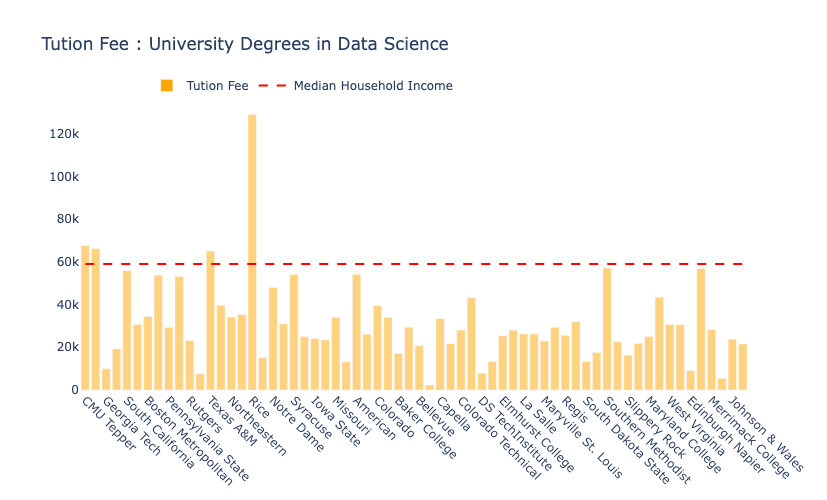
\includegraphics[width=\linewidth]{Figures/Outputs/tution-fees.png}
    \caption[Tution fees]{Tuition-fees.}
    \label{fig:figure-03}
\end{figure}
\newpage
\begin{figure}[!htpb]
    \centering
    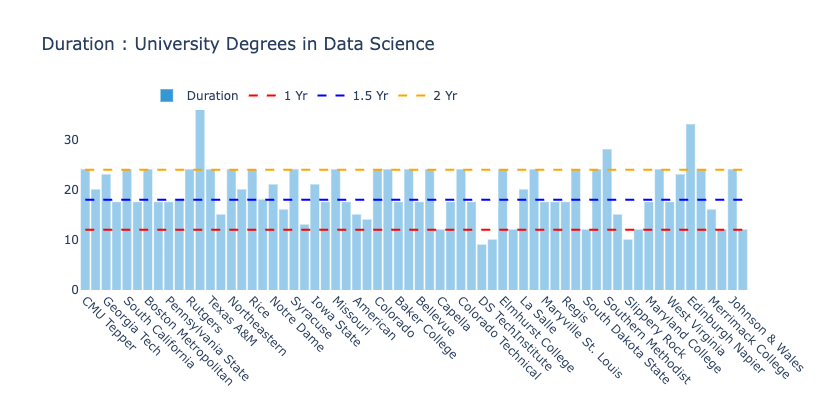
\includegraphics[width=\linewidth]{Figures/Outputs/duration.png}
    \caption[Duration]{Duration.}
    \label{fig:figure-04}
\end{figure}

Time and money are the two biggest investments associated with university degrees. The graph shows that the tuition fee for most of these courses is not cheap and the duration can range from anywhere 1 to 3 years depending upon specialization, location, and university type.

The university courses are of two types:
\begin{itemize}
    \item \textbf{Generic courses} are typically very comprehensive, they cover all parts of data science but they are not very deep and detailed. These type of courses are good for those who want to get acquainted with main elements of this field.
    \item The \textbf{specializations}, on the other hand, aim to cover every possible detail of one particular area. They are generally very deep.
\end{itemize}   
For both types of courses, the investment of money and time are always higher as compared to the alternative free ones. 
\begin{importantbox}
    Head of Data Science from Restaurant Technologies, Inc. \href{https://www.kdnuggets.com/2014/06/masters-degree-become-data-scientist.html}{shared}, "No single Masters Program could cover all the disciplines needed in significant depth for one to be an expert in all these areas. Selecting an area or two or three and having depth and expertise in those is common. Many companies do not have just a "Data Scientist" but teams comprised of experts from the different disciplines."
\end{importantbox}

\section{Proportion of Individuals with University Degrees}
Let's look at what per cent of individuals completed their university degrees to become a data scientist across different countries. Respondents were asked about their country in one of the questions.
\begin{figure}[!htpb]
    \centering
    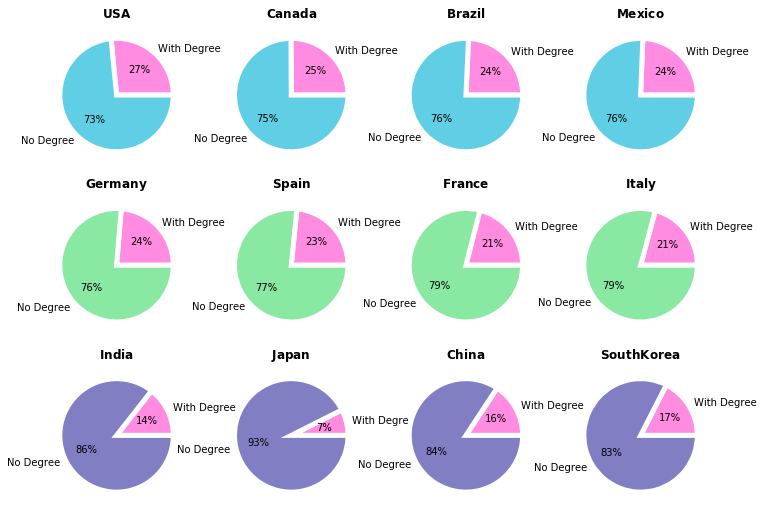
\includegraphics[width=\linewidth]{Figures/Outputs/prop-of-uni-students.png}
    \label{fig:figure-05}
\end{figure}
\subsubsection{Key Findings}
\begin{enumerate}
    \item In the American continent, the USA and Canada are the two most sought places to pursue higher education degrees. About one-fourth of the respondents from these countries have completed their university degrees to becoming a data scientist. In the United States, about 27\% of the individuals who were part of this survey completed their university degrees. In Europe, there are about one-fifth of respondents who completed their university degrees while in Asia, the percentage is a bit lower only about 15\%.
    \item Countries with the highest proportion of data scientists with university degrees are \textbf{'Tunisia'}, \textbf{'Austria'}, \textbf{'New Zealand'} and \textbf{'Greece'} with \textbf{over 40\% of the individuals completing university degrees}. On the other hand, countries \textbf{'Japan'}, \textbf{'Nigeria'}, \textbf{'Belarus'}, and \textbf{'Algeria'} shows a lower number (less than 10\%) of individuals completing university degrees.
    \item Among the genders, female respondents have a higher number for completing university degrees than male respondents. \textbf{23\% of the female respondents} and 20\% of the male respondents completed their university degrees.
\end{enumerate}